\documentclass{article}

\usepackage[utf8]{inputenc}
\usepackage[english]{babel}

\usepackage{amsmath,amsfonts,amssymb}
\usepackage{fullpage}
\usepackage{verbatim}
\usepackage{mathabx}

\usepackage{tikz,pgfplots}

\pgfplotsset{
  width=150mm,height=100mm,
  major grid style={thin,dotted,color=black!50},
  minor grid style={thin,dotted,color=black!50},
  grid,
  every axis/.append style={
    line width=0.5pt,
    tick style={
      line cap=round,
      thin,
      major tick length=4pt,
      minor tick length=2pt,
    },
  },
  legend cell align=left,
  legend pos=north west,
}

%%%%%%%%%%%%%%%%%%%%%%%%%%%%%%%%%%%%%%%%%%%%%%%%%%%%%%%%%%%%%%%%%%%%%%%%%%%%%%%%

\begin{document}

\title{LCE-Queries}
\author{Alexander Herlez}
%\maketitle



% IMPORT-DATA stats time.txt-2019-05-01-22-44-54

\begin{center}
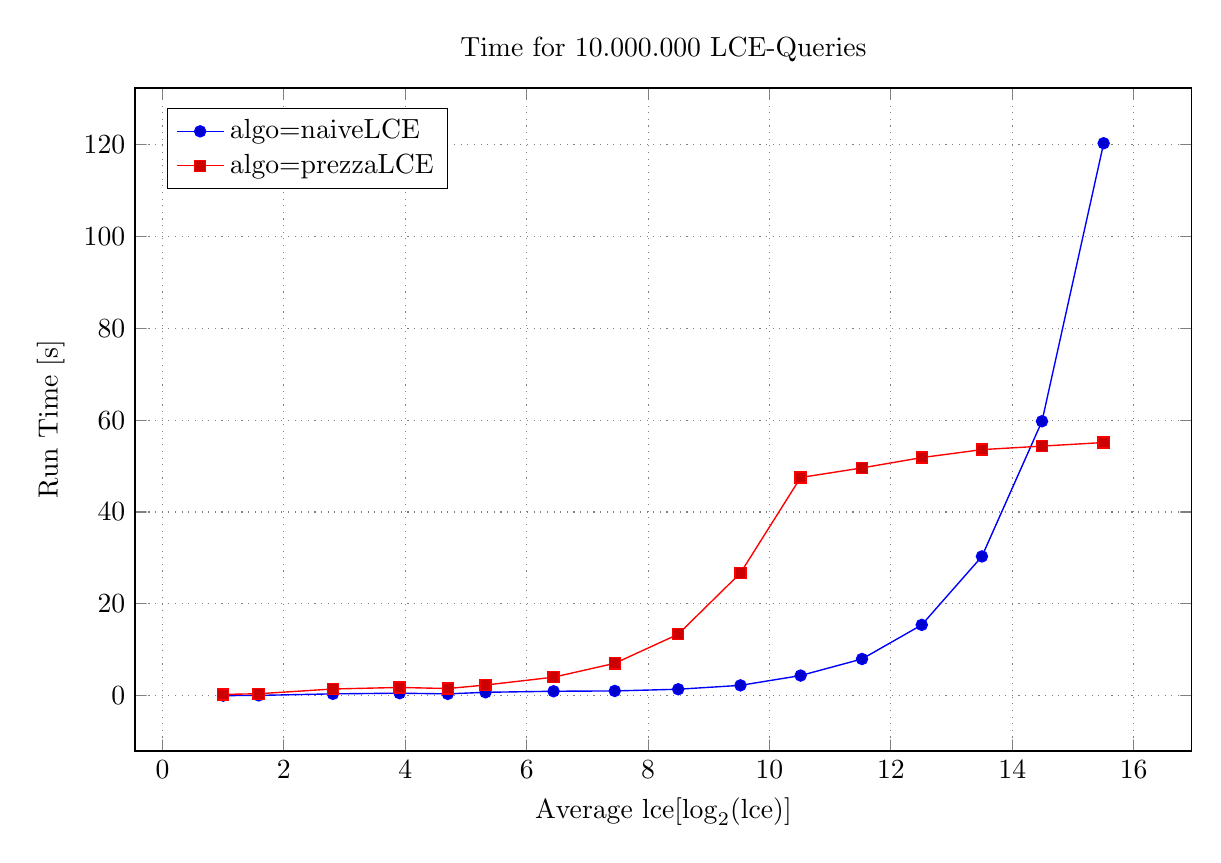
\begin{tikzpicture}
  \begin{axis}[
    title={Time for 10.000.000 LCE-Queries},
    xlabel={Average lce[$\log_2$(lce)]},
    ylabel={Run Time [s]},
    ]

    %% MULTIPLOT(algo) SELECT LOG(2, aveLCE) AS x, time AS y, MULTIPLOT
    %% FROM stats GROUP BY MULTIPLOT,x  ORDER BY MULTIPLOT,x
    \addplot coordinates { (1.0,0.031718) (1.58496,0.0834501) (2.80735,0.419115) (3.90689,0.566483) (4.70044,0.412786) (5.32193,0.759189) (6.44294,0.985373) (7.45121,1.05472) (8.49586,1.42359) (9.5216,2.26951) (10.5127,4.40452) (11.5241,8.01095) (12.5085,15.435) (13.4995,30.3342) (14.4891,59.7629) (15.505,120.273) };
    \addlegendentry{algo=naiveLCE};
    \addplot coordinates { (1.0,0.297094) (1.58496,0.444572) (2.80735,1.47916) (3.90689,1.81489) (4.70044,1.57609) (5.32193,2.34053) (6.44294,4.04676) (7.45121,7.06974) (8.49586,13.3987) (9.5216,26.7269) (10.5127,47.5142) (11.5241,49.5999) (12.5085,51.8503) (13.4995,53.582) (14.4891,54.3478) (15.505,55.1325) };
    \addlegendentry{algo=prezzaLCE};

  \end{axis}
\end{tikzpicture}
\end{center}

\begin{center}
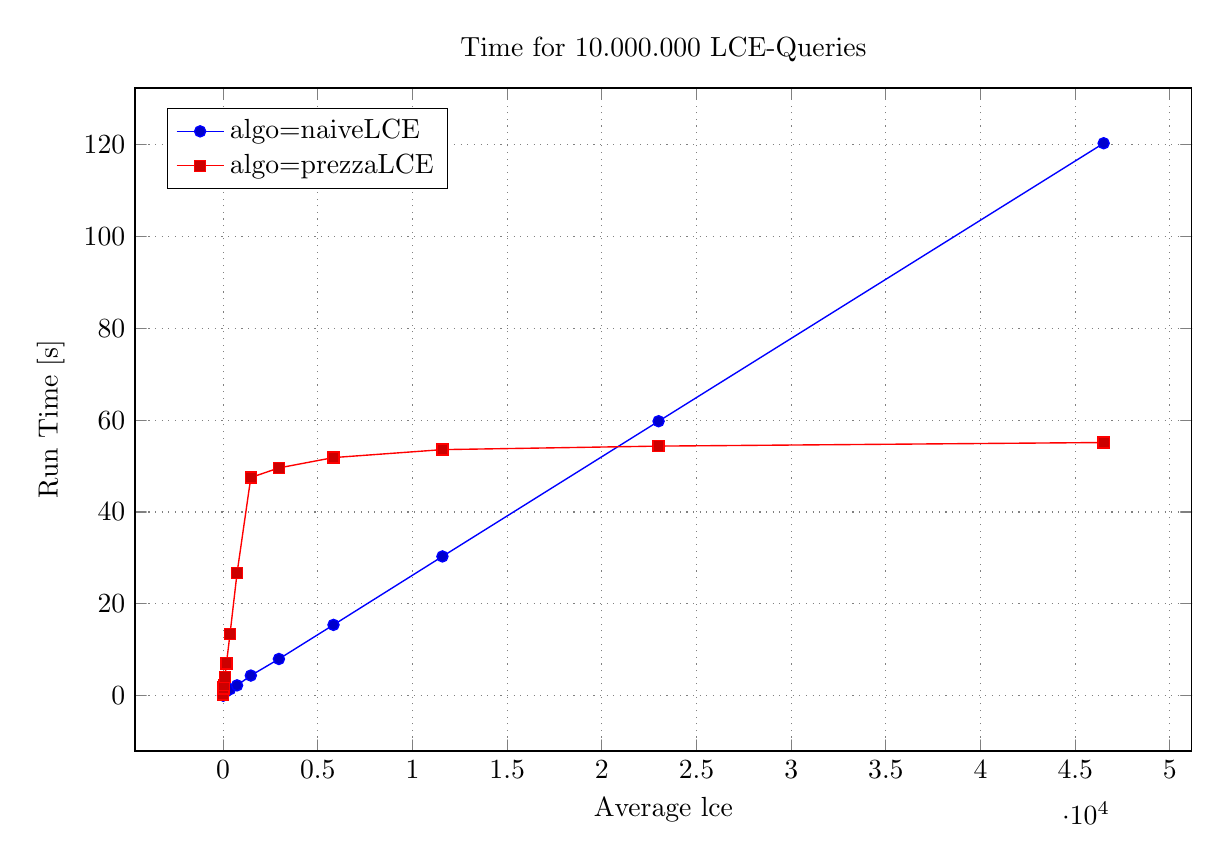
\begin{tikzpicture}
  \begin{axis}[
    title={Time for 10.000.000 LCE-Queries},
    xlabel={Average lce},
    ylabel={Run Time [s]},
    ]

    %% MULTIPLOT(algo) SELECT aveLCE AS x, time AS y, MULTIPLOT
    %% FROM stats GROUP BY MULTIPLOT,x  ORDER BY MULTIPLOT,x
    \addplot coordinates { (2,0.031718) (3,0.0834501) (7,0.419115) (15,0.566483) (26,0.412786) (40,0.759189) (87,0.985373) (175,1.05472) (361,1.42359) (735,2.26951) (1461,4.40452) (2945,8.01095) (5827,15.435) (11581,30.3342) (22996,59.7629) (46502,120.273) };
    \addlegendentry{algo=naiveLCE};
    \addplot coordinates { (2,0.297094) (3,0.444572) (7,1.47916) (15,1.81489) (26,1.57609) (40,2.34053) (87,4.04676) (175,7.06974) (361,13.3987) (735,26.7269) (1461,47.5142) (2945,49.5999) (5827,51.8503) (11581,53.582) (22996,54.3478) (46502,55.1325) };
    \addlegendentry{algo=prezzaLCE};

  \end{axis}
\end{tikzpicture}
\end{center}




\end{document}
